%to do
\section{background}
\label{sec:background}
\subsection{cloud computing}
\begin{figure}
\centering
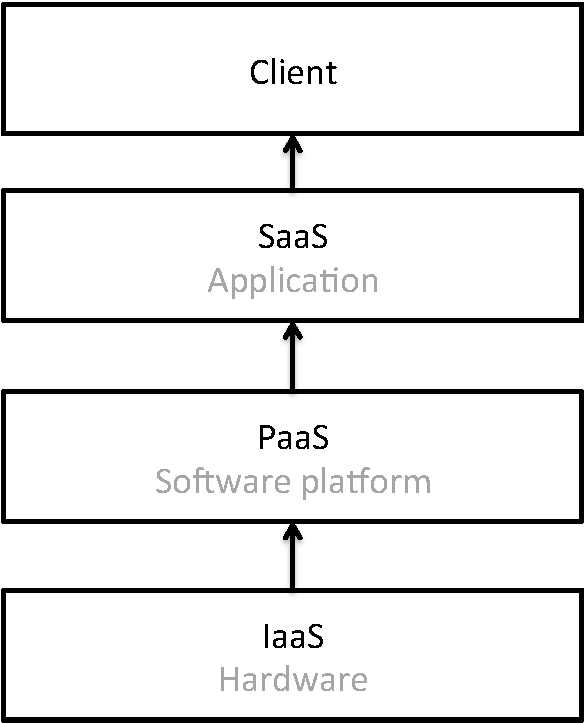
\includegraphics[width=4cm]{img/cloud_models}
\caption{the relationship of different cloud models}
\label{background:cloud models}
\end{figure}

Cloud computing refers to a model that cloud vendors provide user IT resources and charge them for
the resources they used.
Cloud vendors can offer hardware resources including CPU, memory, hard disk, network and software
resources OS, software suits and applications.
Cloud computing majorly can be classified into following three kinds of models:
\begin{enumerate}
  \item Infrastructure as a service (IaaS): cloud vendors provide only raw machines(physical or
  virtual machine), user need to set up the whole software environment including OS.
  \item Platform as a service (PaaS): in this model, cloud vendors provide hardware as well as
  software platform. Users can use it as a common computer and run applications on the platform.
  Amazon EC2 provides PaaS.
  \item Software as a service (SaaS): Cloud vendors provide a certain applications. Users don't need
  to configure the software themselves.
\end{enumerate}
The relationship of different cloud models can be shown as Figure~.\ref{background:cloud models}

Cloud computing can have following benefits:
\begin{itemize}
  \item User don't need to care about the machine placement and maintenance.
  \item User don't need a large number of machines to meet a temporally request peek and idle for
  the other time, Since cloud instances can set up in a few minutes when the request peek occurs.
  \item User don't need to pay for expensive hardware and software, they just need to pay for what
  they used.
\end{itemize}

\subsection{burst buffer}
Modern high performance systems consist of thousands of compute nodes, and hundreds of
applications are running at the same time, these applications require for around 80GiB/s of
bandwidth and the demand are expected to have TiB level in the near future.
Also The shared storage
systems can easily become the bottleneck of the whole system\xtq{citation},


